\documentclass[]{jsarticle}
\usepackage[dvipdfmx]{graphicx}
\usepackage[deluxe]{otf}
\usepackage[hang,small,bf]{caption}
\usepackage[subrefformat=parens]{subcaption}
\captionsetup{compatibility=false}

\renewcommand{\kanjifamilydefault}{\mgdefault}
\newcommand*{\graphc}[3][7.0cm]{\begin{figure}[h] \begin{center}\includegraphics[clip,width= #1]{#2}\caption{#3}\end{center}\end{figure}}
% http://www.ai.soc.i.kyoto-u.ac.jp/~matsubara/le4-2016/index.php?%28Step1%29%20SVM%E3%81%AE%E4%BD%9C%E6%88%90


\begin{document}
\title{平成28年度 3回生後期実験(エージェント) \\ 課題3 SVRの作成 }
\author{村田 叡}
\date{ 2016/11/4 }
\maketitle

\section{プログラム概要}
今回の課題では、SVRのプログラムを作成した。
データファイルを読み込み、回帰式を出力することができる。
また、引数を変えれば交差検定を行うこともできる。
以下にその詳細を述べる。


\subsection{実装言語の変更について}
前回までのSVRで提出した課題は全てPython3で実装していたが、
速度に不満を感じたため、プロッティング部分はPython3に任せ、
計算のコアの部分はC++14で実装しなおした。
SVMもPython3からC++14に書き直した時に、
Clang++による最適化(O3),並列化 などの要素により、
目安としてサンプルデータでの交差検定が16倍速くなったので、
C++14にて書く価値はあると判断した。
なおSVMの部分については、今回のレポートには関係がなく、
また、Python3のものとほとんど同様のインターフェースのため省略する。

\subsection{プログラムの起動方法及び実行例}
readme.md  の項 requirements を参照のこと

\section{外部仕様}
プロッティングとデータ抽出にはPython3を、
計算のコア部分にはC++14を用いている。
以下、そのプログラムのCUIについて述べる。

\subsection{py3/plotdata.py}
このコードは datファイル(形式は実験のデータ通り)を読み込み、
そのデータをプロットすることに特化したコードである。
--1d は一次元データを折れ線グラフでプロットし、
--2d はSVM用の二次元データを、
--3d は二次元データを三次元散布図でプロットする。
--save オプションをつけると、結果の画像ファイルを保存できる。
ファイルを2つ指定して、2つのデータを重ねて表示して差異を確認することもできる。
実際の使用例は、readme.md の項 example を参照のこと。

\subsection{実行可能ファイル svr}
このファイルは datファイルを読み込み、SVRを作成する。
--plot オプションをつけると、結果をdatファイル形式で出力し、
--cross オプションをつけると、交差検定を行う。
--p, --c, --eps オプションを指定して、値を指定することができる。
gauss, polynomial, linear などを引数に入れておくことでカーネル指定することができる。
mean\_abs,mean\_square,coefficient などを引数に入れておくことで、
交差検定の指標を指定することができる。
実際の使用例は、readme.md の項 example を参照のこと。


\section{内部仕様}
全体的にコードが多いので、各ファイルの概要のみを述べる。

\subsection{py3/plotdata.py}
docoptを用いてコマンドライン引数を解析し、
numpyを用いてデータをプロットできる形式に変換し、
matplotlibを用いて実際にデータをプロットしている。


\subsection{cpp/util.*}
このSVRのプロジェクトファイル全体で使用されうるファイルである。
標準ライブラリのインクルード、parse\_args 関数、
最頻の標準関数のusing、どうしても使いたいマクロ3種(REP,FOR,ALL)の定義を行う。
マクロの使用は本来絶対やめるべきだが、個人的コード群であり、
REP.FOR,ALL マクロの有用性は非常に高いため、使用することにした。
(マクロの使用については、例えばquadProg++ 自体に,\verb|#define solve lu_solve|など
が書いてあり、(しかもundefしていない)solveという名前が文脈に関係なく
一生使えないようになっていたりしたので、私はquadProg++の作成者に強い憤りを感じた。)
\subsubsection{ parse\_args関数 }
この関数はコマンドライン引数のパースを行う。
この関数は、SVMを作成する際のmain関数からも参照されうるため、範囲の広いところで定義をした。
コマンドライン引数に、所望するキーワードが入っているか、
入っていればそのパラメータは何かを解析する。


\subsection{cpp/kernel.*}
このファイルは、クラスKernelを定義する。
Kernelクラスは、内積(linear)、ガウスカーネル(gauss)、多項式カーネル(polynomial)の
カーネルを表現するクラスである。
\verb|enum Kernel::kind| を内包し、それに応じたカーネルを提供する。
コンストラクタにて Kernel::kind 及び パラメータ(例えばガウスカーネルならσ)をとり、カーネルを確定させる。
自身のカーネルの文字列型との変換関数(to\_string / strings2kernel\_kind)も提供する。
また、データ全体に適用する関数群についてもこのクラスのstatic関数としており、
例えば、ファイルからデータを読み込むread\_data関数、
読み込んだデータを0から1の範囲に正規化するnormalize関数などを提供している。


\subsection{cpp/plotable.h}
このクラスは、プロットできる関数に対する基底クラスである。
プロットできる関数として、ここではSVMやSVRなどが該当する。
実際にSVRクラス、SVMクラスはこのクラスを継承する。
このクラスは抽象メソッドとして
\verb|virtual double func(const vector<double> &x) const|を
もつクラスが継承できる。
このfuncメソッドを利用して、指定したファイルに、1次元又は2次元のデータを
グリッド状にプロットするplot\_data関数を実装しているため、
このクラスを継承しているSVRやSVMクラスではplot\_data関数を利用することができる。

\subsection{cpp/main.cpp}
このファイルは、メイン関数を提供する。
コマンドライン引数の解析を行い、print\_usage関数を使用して使用方法をアラートしたり、
実際にデータを正規化したのちSVRに投げたり、交差検定を行ったり、プロットしたりする。

\subsection{cpp/svr.*}
このファイル群にてSVRクラスを実装している。
\subsubsection{SVRクラス}
このクラスは、SVRを表現する。
コンストラクタにて、サンプルデータ点 x,およびその値 y,
パラメータが確定したカーネル、C、epsというSVRを形成に必要十分なデータを取り、
実際にsolve関数にてSVRを解く。
quadProg++を用いてSVRを解き、サポートベクターとなっている点からθを計算し、評価器を得る。
サポートベクターの数だけ微小に異なるθが存在するが、中央値のθをとることにした。
評価器を得た後は、そのインスタンスはfunc関数、print\_func関数、test関数を提供できる。
func関数は、実際の評価器を表現し(内部で関数kernel\_dot\_to\_wを使用する)、
print\_func 関数は、その評価機を出力する。
test関数は、その評価器の精度の目安として、その評価器を使用した値と実際の値の差がeps内に
あるサンプル点の割合をプリントする。
\subsubsection{SVRクラスの交差検定}
SVRクラスはstatic関数として、
交差検定を行うcross\_validation関数、及び
それを利用してパラメータやCの値を探索する search\_parameter関数を提供する。
cross\_validation関数についてはSVMの時に実装したものとほとんど同じである。
但し、指標として正解数ではなく誤差の総和を持ちる点が異なる。
誤差を計算するために、\verb|enum cross_validation_type | を提供していて、
平均二乗誤差、平均絶対誤差、決定係数などを用いてcalc\_diff関数にて誤差を計算する事ができる。
search\_parameter関数についてもSVMのときのものとほとんど同じであるが、
パラメータに加えてCの値も探索する必要があるため、二次元グリッド上を探索する必要がある
点が異なる。計算量が増えるため、SVMほど詳細に探索できないことが難点である。
ちなみに、計算過程においては高速化を図るため、std::threadを用いて並列化して計算している。

\newpage
\section{考察}
以下では実際に上記のプログラムを用いて、
予測精度がカーネル及びパラメータによりどのように変化するかの考察を行う。
以下では、特に断りが無い限りeps=0.01としている。
\subsection{探索過程の可視化}
誤差の総和が少ないほどよりよいものとして探索する。
最初は荒く、徐々に狭くして探索している。
サンプルデータとして、二次元データであるsample20.datを用いた。
\begin{figure}[htbp]
 \begin{minipage}[b]{0.5\hsize}
  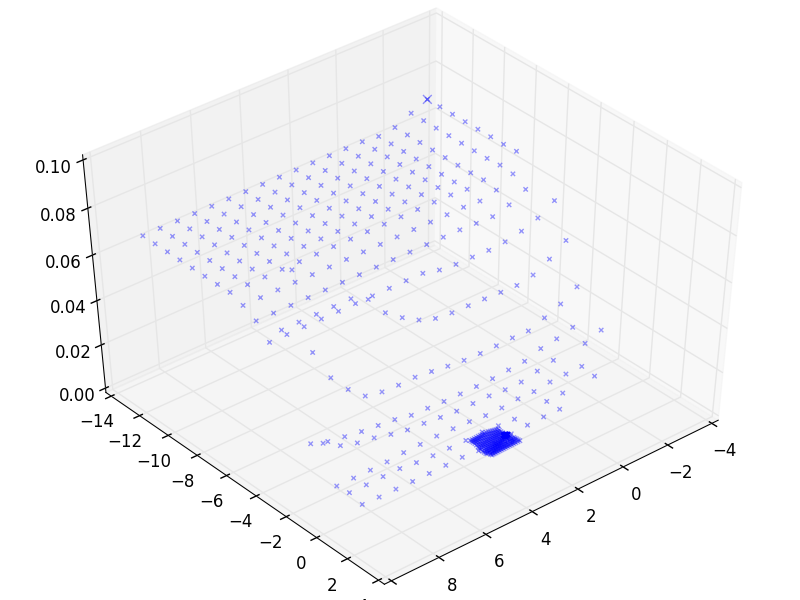
\includegraphics[scale=0.4]{./images/gauss_cross_sq.png}
  \subcaption{平均二乗誤差 ,探索解 $c=6.4663,p=1.72429 $}
 \end{minipage}
 \begin{minipage}[b]{0.5\hsize}
  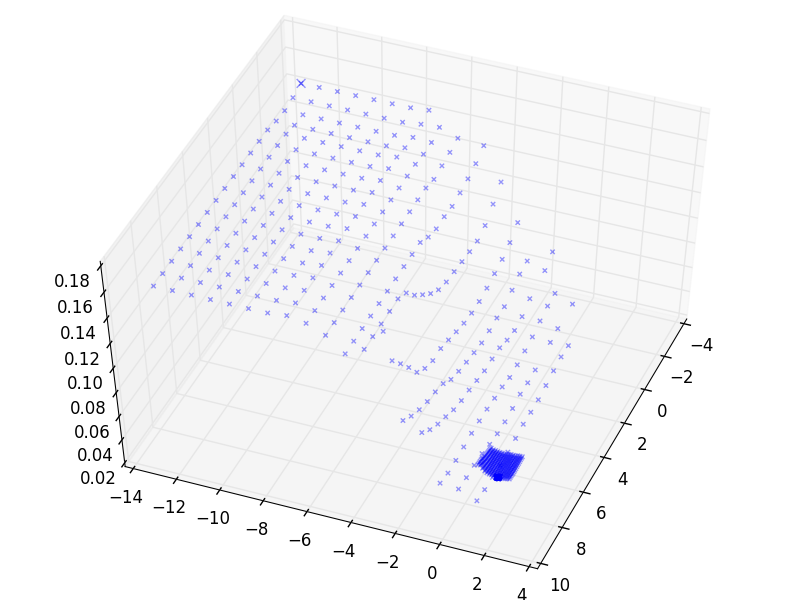
\includegraphics[scale=0.4]{./images/gauss_corss_abs.png}
  \subcaption{平均絶対誤差 ,探索解 $c=186.412,p=2.36526$}
 \end{minipage}
 \begin{minipage}[b]{0.5\hsize}
  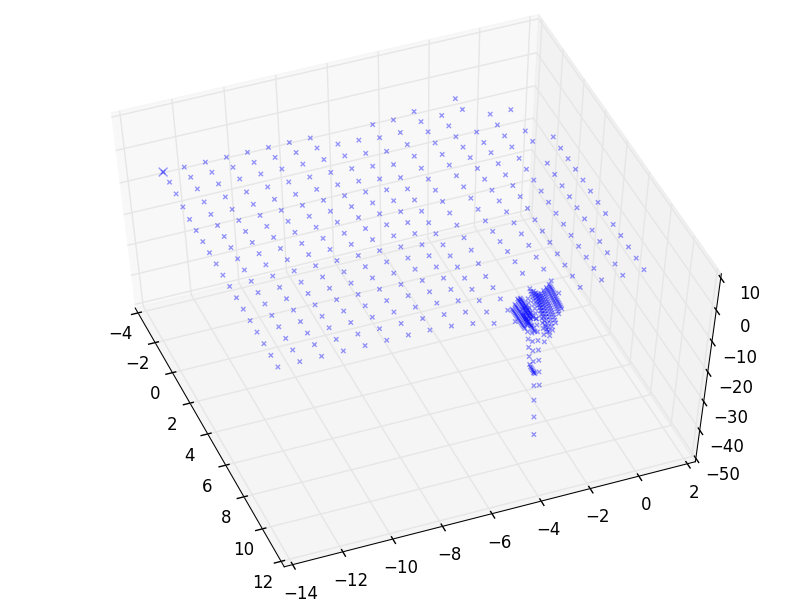
\includegraphics[scale=0.4]{./images/gauss_cross_coef.png}
  \subcaption{決定係数 ,探索解 $c=512,p=0.1152$}
 \end{minipage}
 \caption{ガウスカーネルのパラメータの探索について(グリッドの数値xに対して実際の値は2のx乗を表す)}
\end{figure}

\newpage
\subsection{探索結果の可視化}
二次元データに対してどのように変化するのか容易に確認できるのはPythonの利点である。
\begin{figure}[htbp]
 \begin{minipage}[b]{0.5\hsize}
  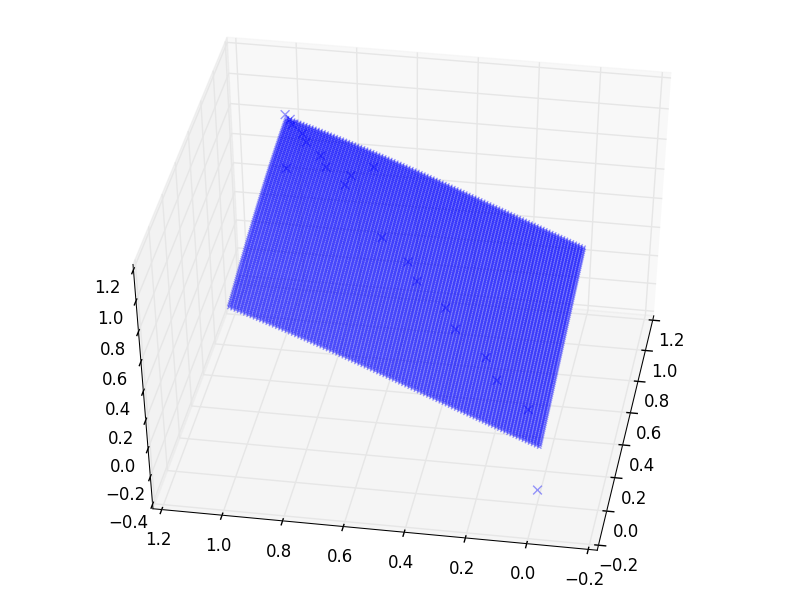
\includegraphics[scale=0.4]{./images/gauss_sq.png}
  \subcaption{平均二乗誤差の探索解 $c=6.4663,p=1.72429 $}
 \end{minipage}
 \begin{minipage}[b]{0.5\hsize}
  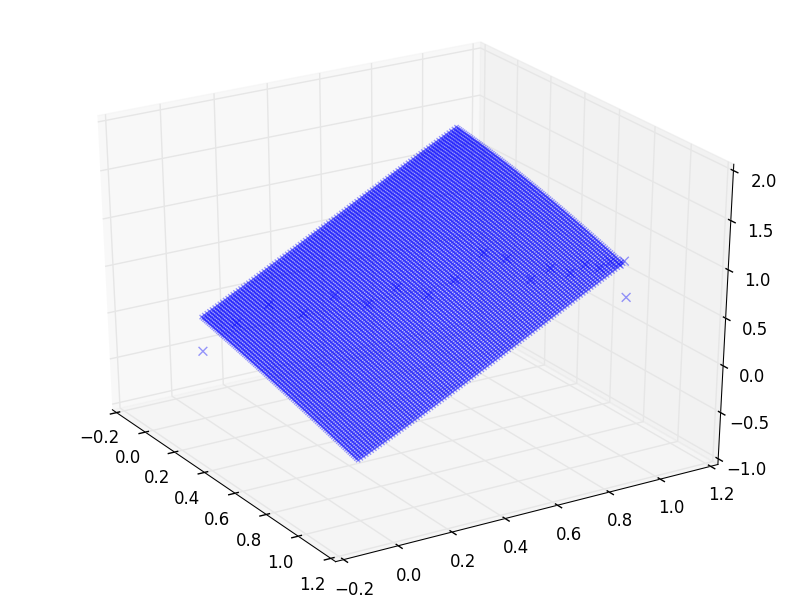
\includegraphics[scale=0.4]{./images/gauss_abs.png}
  \subcaption{平均絶対誤差の探索解 $c=186.412,p=2.36526$}
 \end{minipage}
 \begin{minipage}[b]{0.5\hsize}
  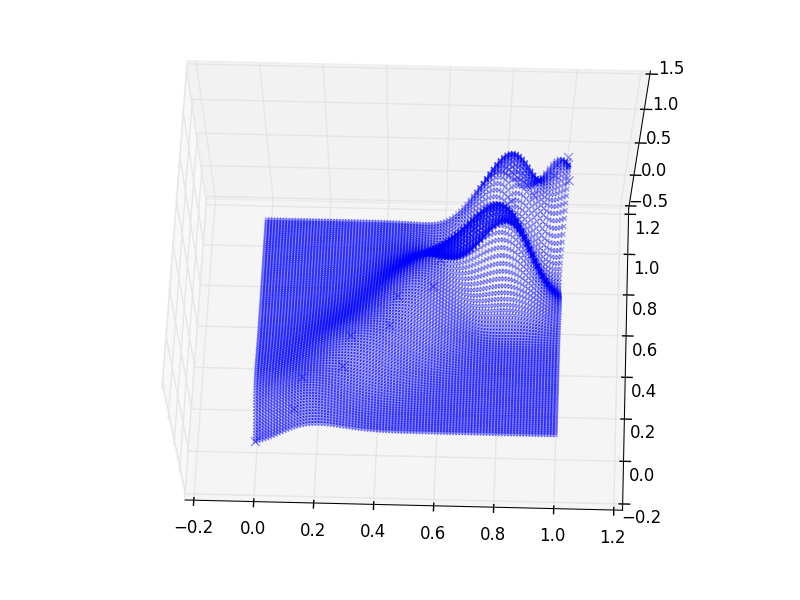
\includegraphics[scale=0.4]{./images/gauss_coef.png}
  \subcaption{決定係数の探索解 $c=512,p=0.1152$}
 \end{minipage}
 \caption{ガウスカーネルのパラメータの探索について(グリッドの数値xに対して実際の値は2のx乗を表す)}
\end{figure}
\newpage

\subsection{ オークションデータの予測について }
課題として与えられたオークションデータを用いて、
カーネルのパラメータとその予測値の変化を可視化する。
実験のページにあるオークションデータは、単純に処理するとサンプルデータ数が10000になり、
とてもではないが計算が間に合わないため、データを別の形式に変換する必要がある。
今回は、日程ごとの差異はなく、時間ごとの差異しかないと仮定して、
同じ時間のデータごとにその中央値のデータを代表点として取り出し、
サンプルデータを96個として予測するものとした。
その処理に関してはpy3/step3\_csv2dat.pyにて実装しているのでそれを参照のこと。
また、オークションのサンプルデータは5つ与えられていたが、
今回の考察ではid0002.csv を使用することにした。
\begin{figure}[htbp]
 \begin{minipage}[b]{0.5\hsize}
  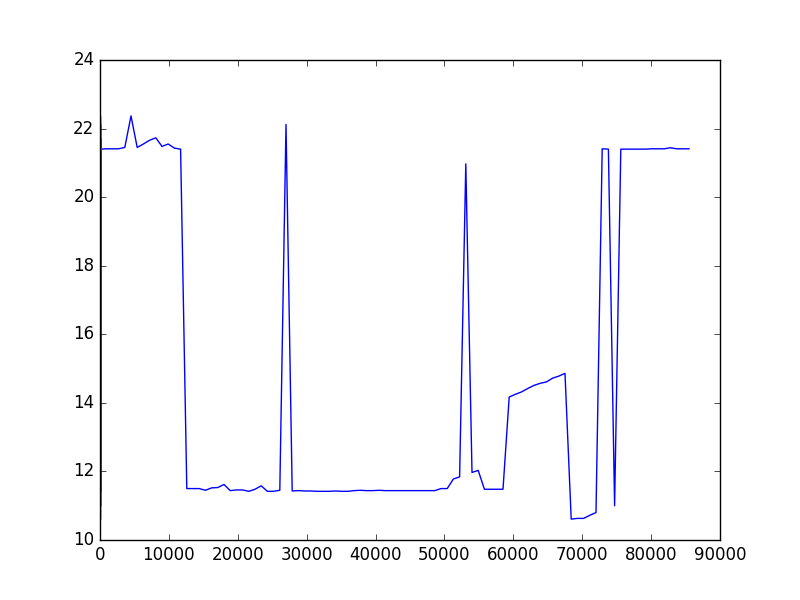
\includegraphics[scale=0.4]{./images/id0001.png}
  \subcaption{id0001}
 \end{minipage}
 \begin{minipage}[b]{0.5\hsize}
  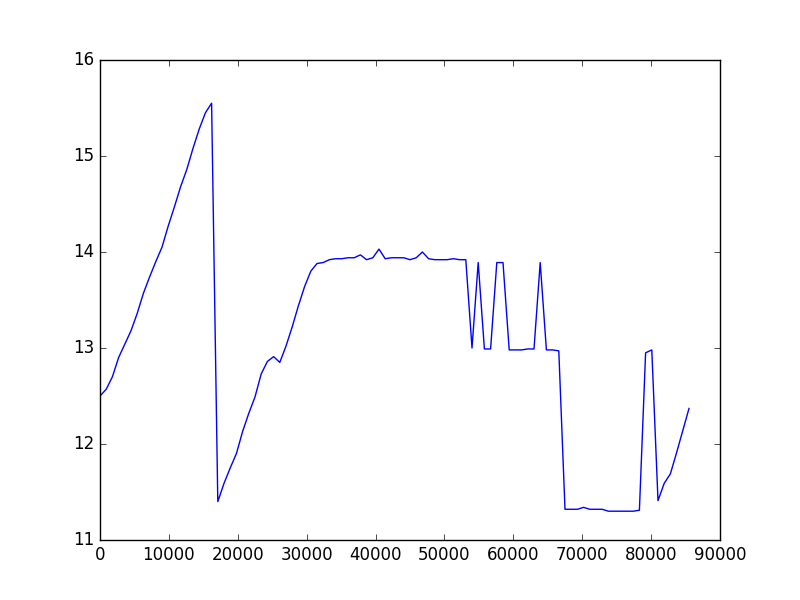
\includegraphics[scale=0.4]{./images/id0002.png}
  \subcaption{id0002}
 \end{minipage}
 \begin{minipage}[b]{0.5\hsize}
  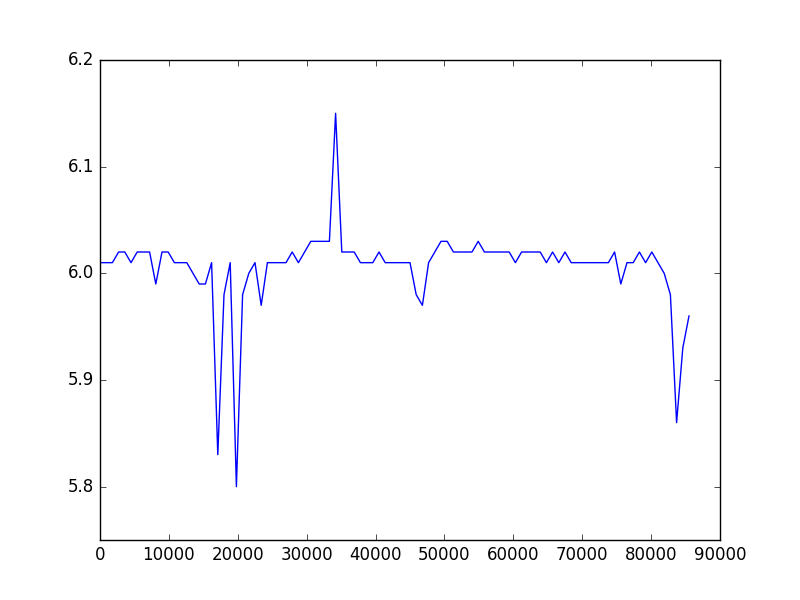
\includegraphics[scale=0.4]{./images/id0003.png}
  \subcaption{id0003}
 \end{minipage}
 \begin{minipage}[b]{0.5\hsize}
  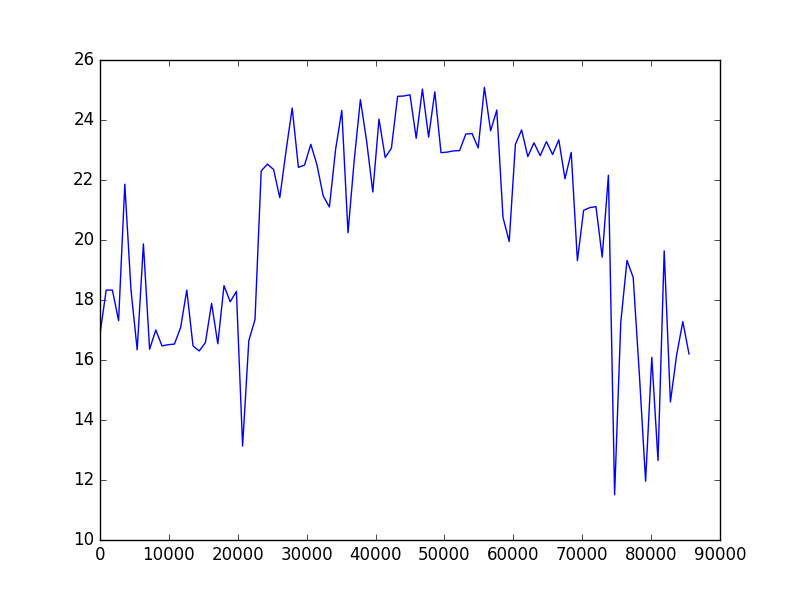
\includegraphics[scale=0.4]{./images/id0004.png}
  \subcaption{id0004}
 \end{minipage}
 \caption{ 与えられたオークションデータ}
\end{figure}
\newpage
\subsection{ id0002のオークションデータの予測について }
実際にパラメータを変化させてどのように予測精度が変化するかを示す。
以下の図で示すように、Cが大きいほど教師データに依存し、
Cが小さいほどモデルは単純になることが分かる。
また、ガウスカーネルの場合、σが大きいほど緩やかに近似し、
σが小さいほど激しく近似することが分かる。
また、多項式カーネルの近似がどうみても適当すぎるように見える(予測精度が悪く見える)
ことについては、原因をよく考える必要があると思われる。

\begin{figure}[htbp]
 \begin{minipage}[b]{0.5\hsize}
  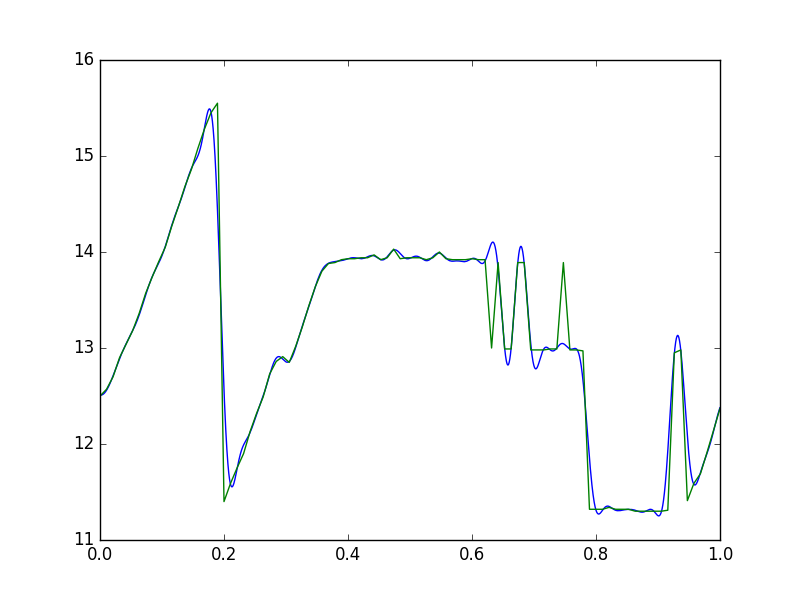
\includegraphics[scale=0.4]{./images/02gauss_sq.png}
  \subcaption{交差検定による結果 $c=81.4532,p0.0207861$}
 \end{minipage}
 \begin{minipage}[b]{0.5\hsize}
  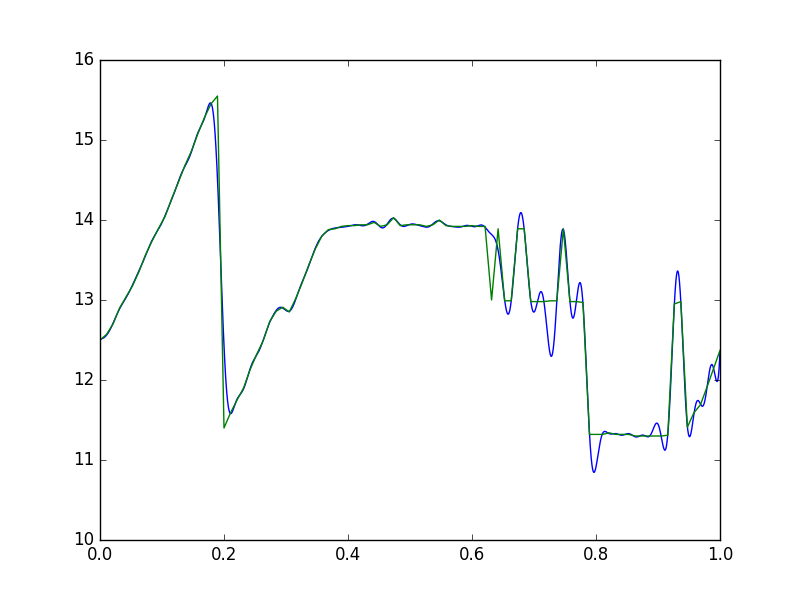
\includegraphics[scale=0.4]{./images/02gauss100c.png}
  \subcaption{Cを100倍してみたもの $c=8145.32,p0.0207861$}
 \end{minipage}
 \begin{minipage}[b]{0.5\hsize}
  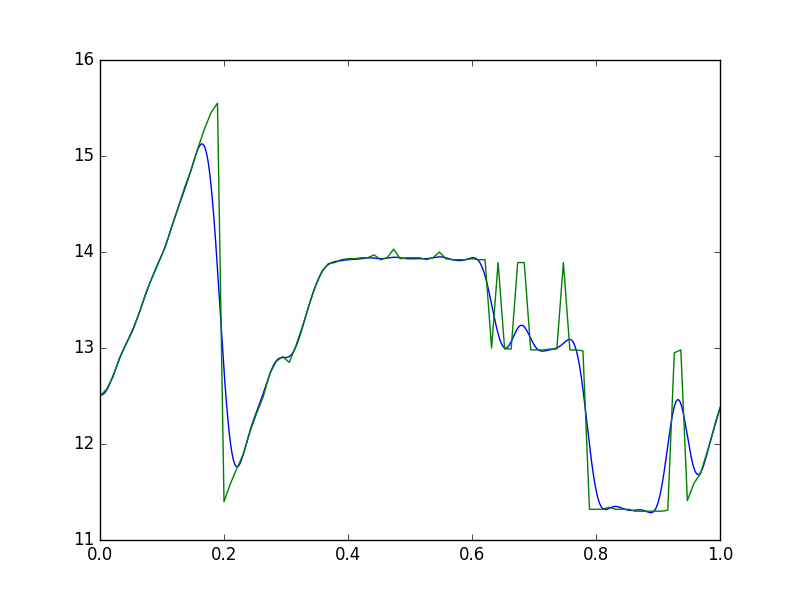
\includegraphics[scale=0.4]{./images/02gauss001c.png}
  \subcaption{Cを0.01倍してみたもの $c=0.814532,p0.0207861$}
 \end{minipage}
 \begin{minipage}[b]{0.5\hsize}
  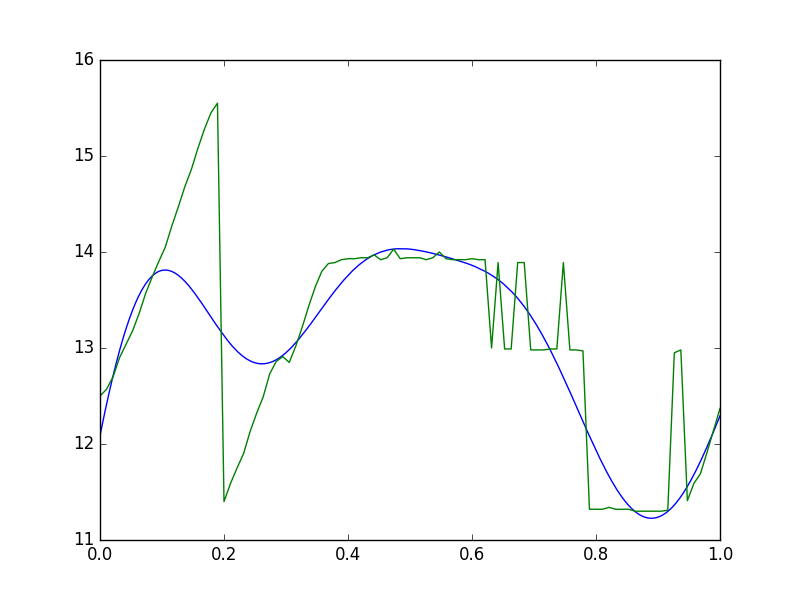
\includegraphics[scale=0.4]{./images/02gauss10p.png}
  \subcaption{σを10倍してみたもの $c=81.4532,p0.207861$}
 \end{minipage}
 \begin{minipage}[b]{0.5\hsize}
  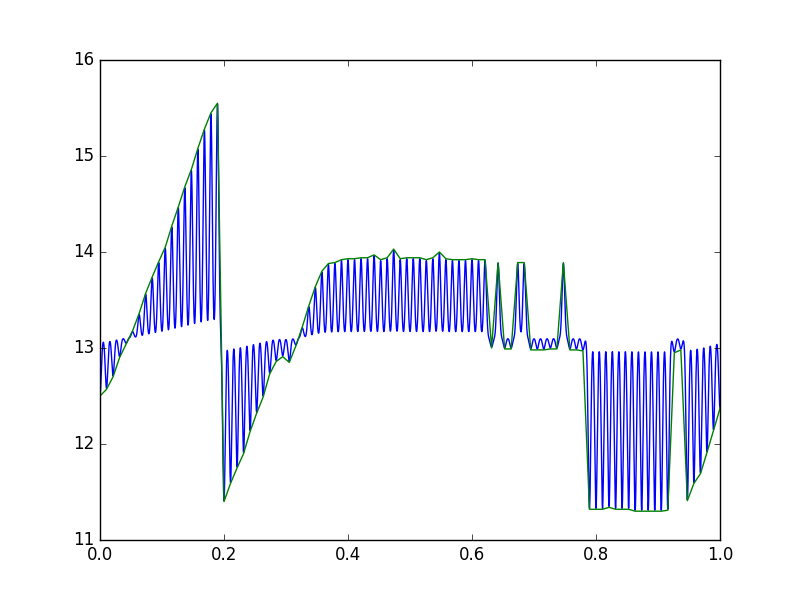
\includegraphics[scale=0.4]{./images/02gauss01p.png}
  \subcaption{σを0.1倍してみたもの $c=81.4532,p0.00207861$}
 \end{minipage}
 \caption{ id0002のガウスカーネルでの変化について}
\end{figure}

\begin{figure}[htbp]
 \begin{minipage}[b]{0.5\hsize}
  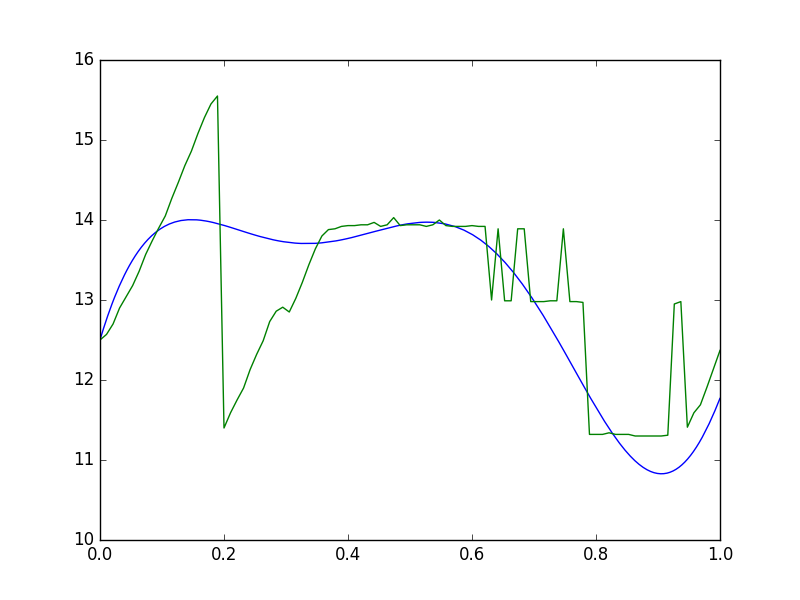
\includegraphics[scale=0.4]{./images/02polym_sq.png}
  \subcaption{交差検定による結果 $c=731.283,p10.6301$}
 \end{minipage}
 \begin{minipage}[b]{0.5\hsize}
  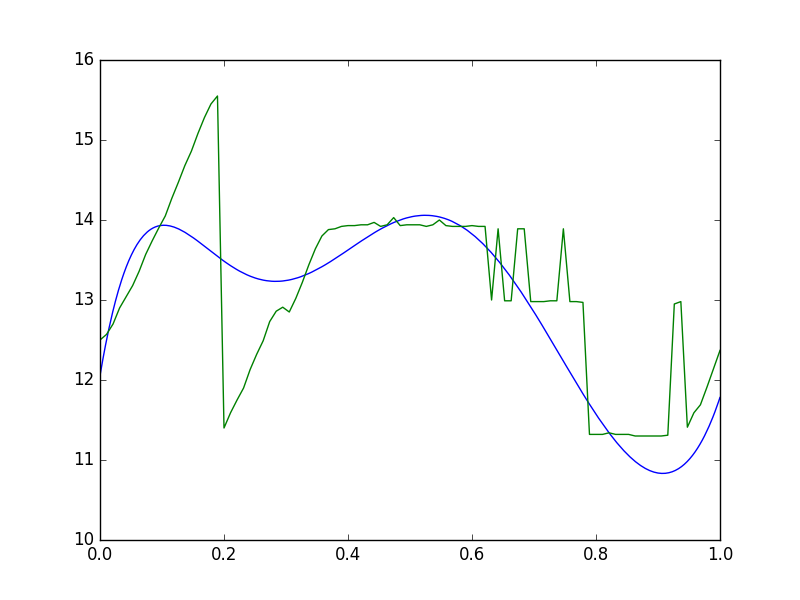
\includegraphics[scale=0.4]{./images/02polym100c.png}
  \subcaption{Cを100倍してみたもの $c=73128.3,p10.6301$}
 \end{minipage}
 \begin{minipage}[b]{0.5\hsize}
  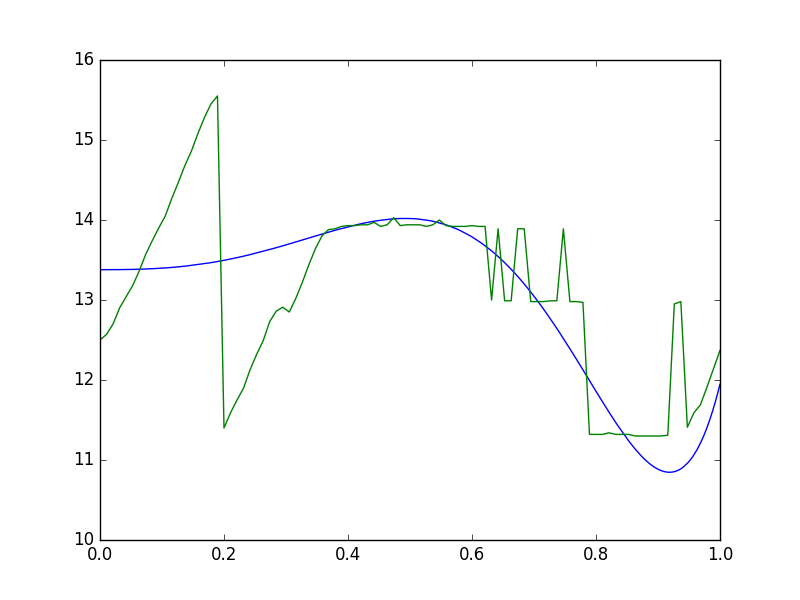
\includegraphics[scale=0.4]{./images/02polym001c.png}
  \subcaption{Cを0.01倍してみたもの $c=7.31283,p10.6301$}
 \end{minipage}
 \caption{ id0002の多項式カーネルでの変化について}
\end{figure}



\end{document}